\subsection{Vision tasks on robots}
Vision tasks play a crucial role in enabling robots to perceive, understand, and interact with the environment. 
Visual information is essential for various robotic tasks, such as object recognition~\cite{galvez2018object}, navigation~\cite{ran2017convolutional}, manipulation~\cite{bayar2018constrained}, and human-robot interaction~\cite{wu2019weight}. 
The rapid advancements in machine learning, particularly deep learning, have revolutionized the field of computer vision and have been widely adopted in robotic applications, which form the foundation for many high-level robotic tasks.

However, the deployment of visual models on resource-constrained robots poses significant challenges. 
Visual models often require significant computational resources and memory, which may not be readily available on robots, especially in mobile and embedded systems. 
Furthermore, real-time performance is critical for many robotic tasks, as robots need to process and respond to visual information quickly to ensure safe and effective operation. 
Therefore, fast visual model inference becomes a key requirement for the successful deployment of deep learning models in robotic applications.
Addressing these challenges is essential for enabling robots to effectively perceive, understand, and interact with their environment in real time, paving the way for more intelligent and autonomous robotic systems.


\subsection{Visual Models}
Convolutional layers~\cite{o2015introduction} have become a fundamental building block in visual models, leading to significant breakthroughs in various computer vision tasks. 
Inspired by the biological structure of the visual cortex~\cite{tripp2019approximating}, these layers apply learnable filters to the input image, performing convolution operations to produce feature maps that highlight the presence of specific patterns at different spatial locations (i.e., local operators). 
This enables deep learning models to capture translation-invariant features and learn hierarchical representations~\cite{ma2015hierarchical}, with early layers learning low-level features like edges and corners, and deeper layers learning more complex patterns and object parts. 
As a result, deep convolutional neural networks (CNNs) have achieved state-of-the-art performance in various vision applications, image classification~\cite{rawat2017deep}, object detection~\cite{galvez2018object}, and semantic segmentation~\cite{wang2018understanding}, due to their ability to effectively capture and learn spatial hierarchies of features from raw input images. 
As the field of computer vision continues to evolve, convolutional layers are expected to remain a crucial component in the development of advanced models for understanding and analyzing visual data.

% Notice that operators for DNN layer (e.g., convolution, ReLU, softmax) can be categorized into two types: local operators and global operators, depending on whether they can be computed independently with partial input according to ~\cite{sun2024hybridparallel}, and the convolutional layer is a typical local operator, as it can be computed with partial input tensor (the blocks in the input tensor for convolution).

\subsection{Resource Limitations of Robots}
In real-world scenarios, robots often navigate and move around to perform tasks such as search and exploration. 
While wireless networks provide high mobility, they also have limited bandwidth, which can significantly impact the performance of robotic IoT systems.
Wireless transmission of robots is constrained by limited bandwidth, both due to the theoretical upper limit of wireless transmission technologies and the practical instability of wireless networks. 
For instance, the most advanced Wi-Fi technology, Wi-Fi 6, offers a maximum theoretical bandwidth of 1.2 Gbps for a single stream~\cite{liu2023first}. However, the limited hardware resources on robots often prevent them from fully utilizing the potential of Wi-Fi 6~\cite{yang2022mobile}. 
Moreover, the actual available bandwidth of wireless networks is often reduced in practice due to various factors, such as the movement of devices~\cite{masiukiewicz2019throughput, pei2013connectivity}, occlusion by physical barriers~\cite{ding2015performance, sarkar2013effect}, and preemption of the wireless channel by other devices~\cite{adame2021time, ren2018proportional}.

To demonstrate the instability of wireless transmission in real-world situations, we conducted a robot surveillance experiment using four-wheel robots navigating around several given points at 5-40cm/s speed in our lab (indoors) and campus garden (outdoors), with hardware and wireless network settings as described in Sec.~\ref{sec:eva}. 
We saturated the wireless network connection with iperf ~\cite{noauthor_iperf_nodate} and recorded the average bandwidth capacity between these robots every 0.1s for 5 minutes.

\begin{figure}[htp]
    \centering
    \subfloat[Indoors\label{fig:indoors}]{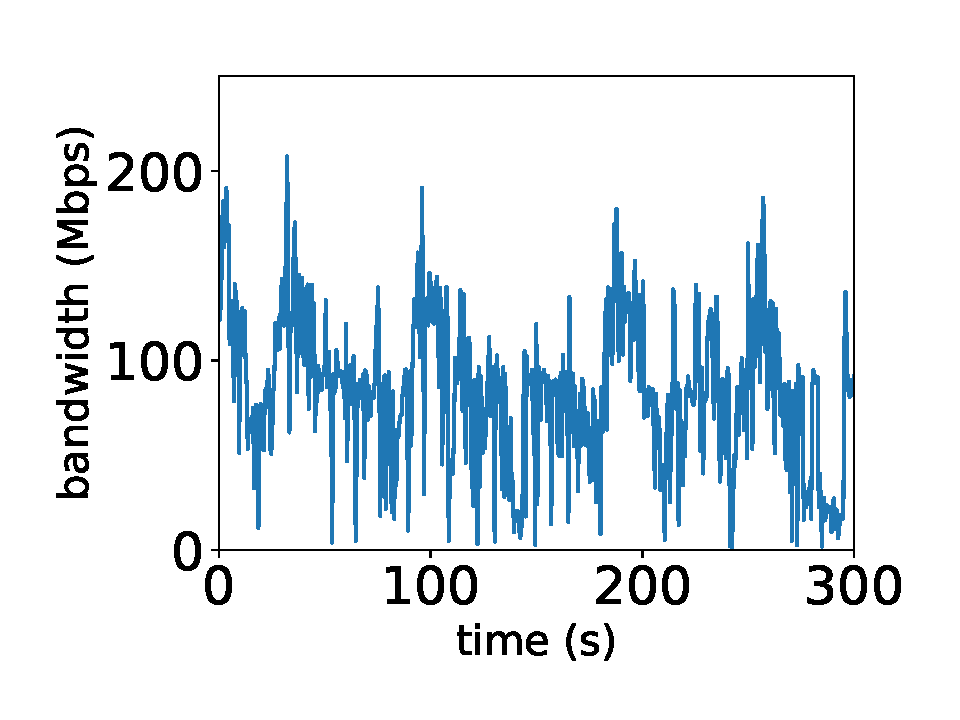
\includegraphics[width=0.48\linewidth]{fig/indoors.pdf}}
    \hfil
    \subfloat[Outdoors\label{fig:outdoors}]{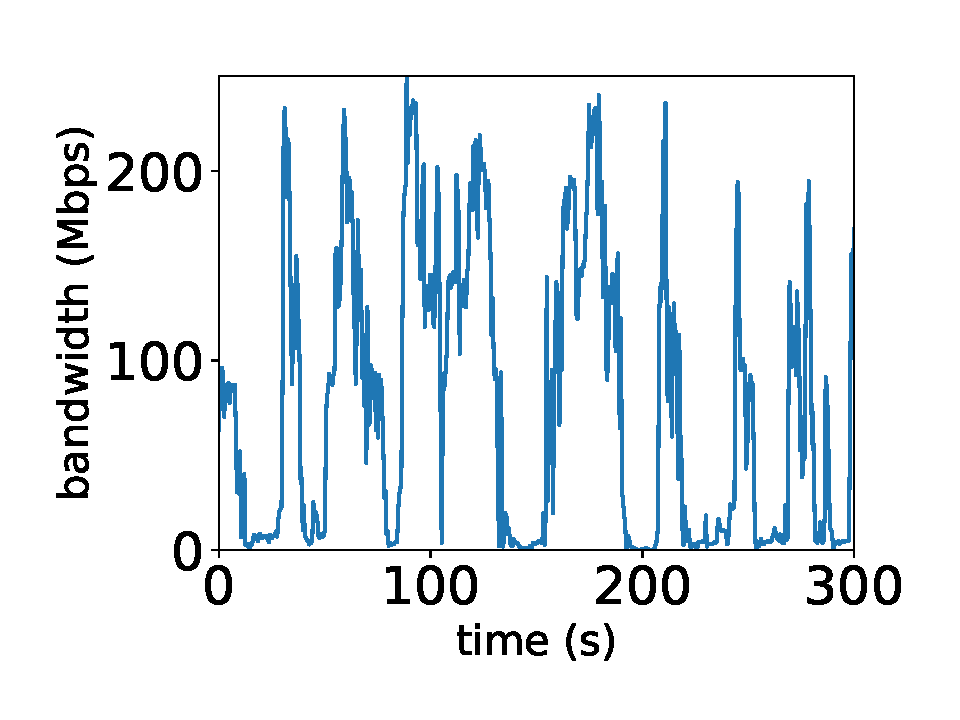
\includegraphics[width=0.48\linewidth]{fig/outdoors.pdf}}
    \caption{The instability of wireless transmission between our robot and a base station in robotic IoT networks.}
    \label{fig:bandwidth} 
\end{figure}


The results in Fig.~\ref{fig:bandwidth} show average bandwidth capacities of 93 Mbps and 73 Mbps for indoor and outdoor scenarios, respectively. 
The outdoor environment exhibited higher instability, with bandwidth frequently dropping to extremely low values around 0 Mbps, due to the lack of walls to reflect wireless signals and the presence of obstacles like trees between communicating robots, resulting in fewer received signals compared to indoor environments. This limitation on the wireless network bandwidth on the robot poses significant challenges for the efficient and reliable computation offloading of robots in real-world scenarios, particularly in outdoor environments where the instability of wireless networks is more pronounced.

\subsection{Related Work}
Edge-Cloud Collaborative Inference expedites the overall inference process by leveraging a GPU server to handle a portion of the computational workload of the robot. 
The DSCCS approach~\cite{liang2023dnn} views the visual model in a layer-wise perspective and focuses on model-layer-level scheduling (layer partitioning) for rapid inference;
Hybrid-Parallel~\cite{sun2024hybridparallel} further offers a more fine-grained control by partitioning and scheduling the computation within local operators, so that the robot can compute on a portion of the input on local operators while at the same time transmitting the result of the input to the GPU server.
It enhances parallelism and further accelerates inference. 
However, despite the advancements in these offloading techniques, the limited bandwidth still poses a bottleneck for data transmission, which our caching mechanism effectively mitigates and achieves a significant improvement in inference performance.

% Cache related (Guan will take it)